% This file was created by tikzplotlib v0.9.1.
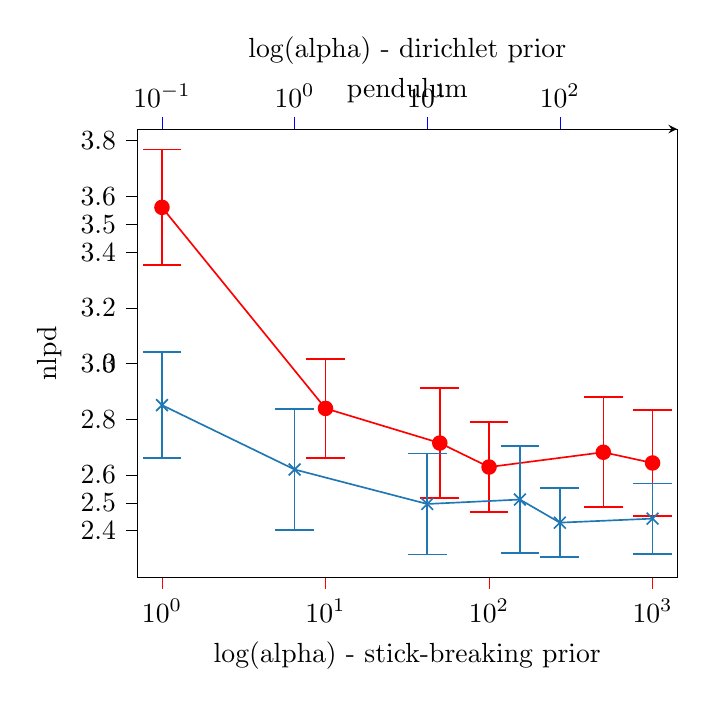
\begin{tikzpicture}

\definecolor{color0}{rgb}{0.12156862745098,0.466666666666667,0.705882352941177}

\begin{axis}[
log basis x={10},
tick align=outside,
tick pos=left,
title={pendulum},
x grid style={white!69.0196078431373!black},
xlabel={log(alpha) - stick-breaking prior},
xmin=0.707945784384138, xmax=1412.53754462275,
xmode=log,
xtick style={color=red},
xtick={0.01,0.1,1,10,100,1000,10000,100000},
xticklabels={\(\displaystyle {10^{-2}}\),\(\displaystyle {10^{-1}}\),\(\displaystyle {10^{0}}\),\(\displaystyle {10^{1}}\),\(\displaystyle {10^{2}}\),\(\displaystyle {10^{3}}\),\(\displaystyle {10^{4}}\),\(\displaystyle {10^{5}}\)},
y grid style={white!69.0196078431373!black},
ylabel={nlpd},
ymin=2.23258959244937, ymax=3.84165363615561,
ytick style={color=black},
ytick={2.2,2.4,2.6,2.8,3,3.2,3.4,3.6,3.8,4},
yticklabels={2.2,2.4,2.6,2.8,3.0,3.2,3.4,3.6,3.8,4.0}
]
\path [draw=red, semithick]
(axis cs:1,3.35277008725353)
--(axis cs:1,3.76851436144169);

\path [draw=red, semithick]
(axis cs:10,2.6609827922019)
--(axis cs:10,3.01715702547952);

\path [draw=red, semithick]
(axis cs:50,2.51850009300761)
--(axis cs:50,2.91119187021493);

\path [draw=red, semithick]
(axis cs:100,2.46786254544317)
--(axis cs:100,2.78943469686902);

\path [draw=red, semithick]
(axis cs:500,2.48463203649059)
--(axis cs:500,2.87888231176845);

\path [draw=red, semithick]
(axis cs:1000,2.45307466672555)
--(axis cs:1000,2.83344496734548);

\addplot [semithick, red, mark=-, mark size=7, mark options={solid}, only marks]
table {%
1 3.35277008725353
10 2.6609827922019
50 2.51850009300761
100 2.46786254544317
500 2.48463203649059
1000 2.45307466672555
};
\addplot [semithick, red, mark=-, mark size=7, mark options={solid}, only marks]
table {%
1 3.76851436144169
10 3.01715702547952
50 2.91119187021493
100 2.78943469686902
500 2.87888231176845
1000 2.83344496734548
};
\addplot [semithick, red, mark=*, mark size=2.5, mark options={solid}]
table {%
1 3.56064222434761
10 2.83906990884071
50 2.71484598161127
100 2.62864862115609
500 2.68175717412952
1000 2.64325981703551
};
\end{axis}

\begin{axis}[
axis x line=top,
log basis x={10},
tick align=outside,
x grid style={white!69.0196078431373!black},
xlabel={log(alpha) - dirichlet prior},
xmin=0.0653208007180445, xmax=765.452956031933,
xmode=log,
xtick pos=right,
xtick style={color=blue},
xtick={0.001,0.01,0.1,1,10,100,1000,10000},
xticklabels={\(\displaystyle {10^{-3}}\),\(\displaystyle {10^{-2}}\),\(\displaystyle {10^{-1}}\),\(\displaystyle {10^{0}}\),\(\displaystyle {10^{1}}\),\(\displaystyle {10^{2}}\),\(\displaystyle {10^{3}}\),\(\displaystyle {10^{4}}\)},
y grid style={white!69.0196078431373!black},
ymin=2.23258959244937, ymax=3.84165363615561,
ytick pos=left,
ytick style={color=black}
]
\path [draw=color0, semithick]
(axis cs:0.1,2.6599567684645)
--(axis cs:0.1,3.04180842219751);

\path [draw=color0, semithick]
(axis cs:1,2.40272277566083)
--(axis cs:1,2.83699793716677);

\path [draw=color0, semithick]
(axis cs:10,2.31503948503447)
--(axis cs:10,2.67714240953498);

\path [draw=color0, semithick]
(axis cs:50,2.31926411445395)
--(axis cs:50,2.70472107168076);

\path [draw=color0, semithick]
(axis cs:100,2.30572886716329)
--(axis cs:100,2.55245214752446);

\path [draw=color0, semithick]
(axis cs:500,2.31755340470602)
--(axis cs:500,2.56948437790584);

\addplot [semithick, color0, mark=-, mark size=7, mark options={solid}, only marks]
table {%
0.1 2.6599567684645
1 2.40272277566083
10 2.31503948503447
50 2.31926411445395
100 2.30572886716329
500 2.31755340470602
};
\addplot [semithick, color0, mark=-, mark size=7, mark options={solid}, only marks]
table {%
0.1 3.04180842219751
1 2.83699793716677
10 2.67714240953498
50 2.70472107168076
100 2.55245214752446
500 2.56948437790584
};
\addplot [semithick, color0, mark=x, mark size=3, mark options={solid}]
table {%
0.1 2.850882595331
1 2.6198603564138
10 2.49609094728473
50 2.51199259306736
100 2.42909050734388
500 2.44351889130593
};
\end{axis}

\end{tikzpicture}
